\documentclass{article}
\usepackage{pgfplots}


\begin{document}
\setlength{\fboxsep}{0pt}
\fbox{
  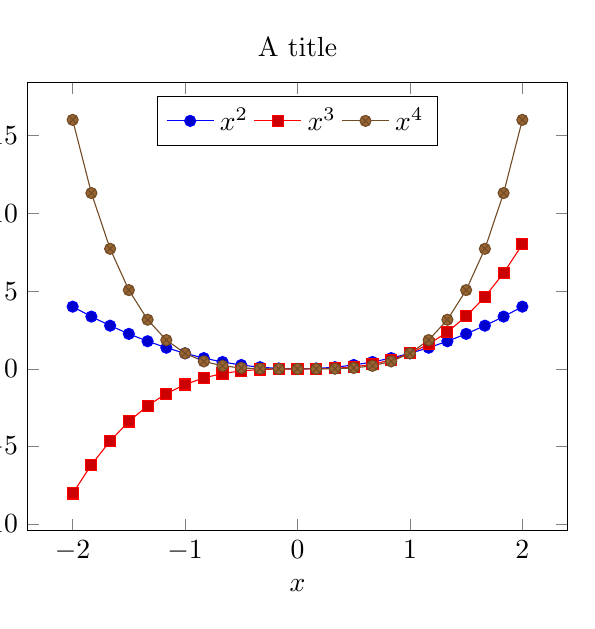
\begin{tikzpicture}
    \begin{pgfinterruptboundingbox}
      \begin{axis}[
          title=A title,
          xlabel={$x$},
          ylabel={$y$},
          legend style={at={(0.5,0.97)},
            anchor=north,legend columns=-1},
          domain=-2:2
        ]
        \addplot {x^2};
        \addplot {x^3};
        \addplot {x^4};
        \legend{$x^2$,$x^3$,$x^4$}
      \end{axis}
    \end{pgfinterruptboundingbox}

    \useasboundingbox
    (current axis.below south west)
    rectangle (current axis.above north east);
  \end{tikzpicture}
  }
\end{document}
